% 第六章正文片段。需在主文件加载 amsmath、amssymb、graphicx。
% 数值由两个独立的 100×4 官方验收表填充，不得从开发样本复制。
\section{问题一与问题二的建模和求解}

\subsection{共同的决策与评价口径}
原始计算图记为 $G=(T\cup O,E)$，其中 $T$ 和 $O$ 分别为张量与操作节点集合。
令 $O^{\mathrm c}=O\setminus\{\mathrm{COPY\_IN},\mathrm{COPY\_OUT}\}$；
对 $o\in O^{\mathrm c}$，$c_o$ 为题面给定的计算周期，$p(o)\in\{M,V\}$
表示其占用的 Cube 或 Vector 管道。张量 $t$ 的大小 $b_t$ 以 byte 计，
逻辑位置由原图的 \texttt{pos} 字段确定。对给定核数 $N\in\{2,3,4,5\}$，
决策是子图映射 $\phi:O^{\mathrm c}\to\mathcal S$、核心分配
$a:\mathcal S\to\{1,\ldots,N\}$ 和每核子图序列 $\pi_k$。

可行方案必须使每个非 COPY 操作恰好属于一个子图、每个子图恰好在一个
$\pi_k$ 中出现一次；原数据依赖形成的子图图为 DAG，序列 $\pi_k$
与其依赖顺序相容。输出文件只含
\texttt{node\_to\_subgraph}、\texttt{core\_schedules} 两个字段。
各核共享同一 DDR 总带宽 $\beta=60\,\mathrm{byte/cycle}$，
私有缓存容量为 $C_{L1}=524288\,\mathrm{byte}$、
$C_{UB}=131072\,\mathrm{byte}$；不能把 $\beta$ 乘以核数。
官方程序在固定配置下计算实际 Makespan $T_{i,N}$ 与总额外 DDR 搬运
$D_{i,N}$。我们以缩短 $T_{i,N}$ 为主，兼顾 $D_{i,N}$。
按题目规定，单核整图调度时间 $T_{i,1}$ 仅作共同参照，
$S_{i,1}=1$，$S_{i,N}=T_{i,1}/T_{i,N}$，
$\bar S_N=100^{-1}\sum_{i=1}^{100}S_{i,N}$。

\subsection{问题一：无核间同步的场景 A}
\subsubsection{Task 边界与计算模型}
场景 A 中一个子图对应一个 Task。任一张量只要跨越子图边界，
即使生产与消费 Task 在同一核心，也必须经 DDR 写回、再读入；
同核两个 Task 切换时私有缓存清空。以 $I_s$、$U_s$ 分别表示
Task $s$ 需从 DDR 读入、向 DDR 写回的不同张量集合，
按 Task 和张量去重后，计划的总搬运量为
\begin{equation}
B_A=\sum_{s\in\mathcal S}\left(\sum_{t\in I_s}b_t+\sum_{t\in U_s}b_t\right),
\qquad D_A=B_A-B_0+B_{\mathrm{spill},A},
\label{eq:chapter6-a-copy}
\end{equation}
其中 $B_0$ 为原图已有的 COPY 字节数，$B_{\mathrm{spill},A}$
是附件核内调度在 L1/UB 不足时实际插入的换出、换入字节数。
式~\eqref{eq:chapter6-a-copy} 区分可由切图直接计数的边界搬运和
只能在正式验收后得到的缓存溢出搬运，避免把二者混作一个预测量。

Task $s$ 在两条计算管道上的工作量分别为
$W_s^q=\sum_{o:\phi(o)=s,\,p(o)=q}c_o$，$q\in\{M,V\}$。
求解时使用的快速时长代理是
\begin{equation}
\widehat d_s^A=\max\left\{W_s^M,W_s^V,
\frac{\sum_{t\in I_s}b_t+\sum_{t\in U_s}b_t}{\beta}\right\}.
\label{eq:chapter6-a-task}
\end{equation}
设 $\mathcal P_A(s)$ 同时包含数据前驱 Task 与同核序列直接前驱；
前者若跨核取等待 $1000$ cycle，后者取 Task 切换等待 $100$ cycle，
其余等待记为 $0$。在依赖与序列的合并 DAG 上递推
\begin{equation}
\widehat F_s^A=\widehat d_s^A+
\max_{r\in\mathcal P_A(s)}\{\widehat F_r^A+\delta^A_{rs}\},
\qquad
\widehat T_A=\max\left\{\max_s\widehat F_s^A,\frac{B_A}{\beta}\right\}.
\label{eq:chapter6-a-proxy}
\end{equation}
空前驱的最大值为 $0$。$\widehat T_A$ 只供候选排序，
并不等于附件的逐 Pipe、多核共享带宽时间线；特别是
$B_{\mathrm{spill},A}$ 不在该代理中。

\subsubsection{零割集装箱与有界结构切分}
首先将计算依赖图的弱连通分量 $C_j$ 作为不可切的装箱物品。
记 $w_j^q=\sum_{o\in C_j,\,p(o)=q}c_o$，$L_k^q$ 为核心 $k$
已分配的对应管道负载。按 $\max_q w_j^q$ 降序遍历分量，
每步选取下式字典序最小的核心：
\begin{equation}
k_j=\arg\min_{k}\left(
\max\{L_k^M+w_j^M,L_k^V+w_j^V\},\;
L_k^M+L_k^V,\;k\right).
\label{eq:chapter6-a-lpt}
\end{equation}
该构造在分量内部不产生通信割，但单个大分量可能独占一核。
式~\eqref{eq:chapter6-a-lpt} 是双管道贪心规则；经典标量 LPT
的完工时间近似界不能直接用于含依赖、DDR 争用和缓存换入换出的本题。
因此仅对原图结构生成有限种补充方案：按图深划带、在宽度谷处分段、
在汇合点前后区分分支、按共享祖先或后继关系聚合。
对最大拓扑深度 $h$ 和总计算工作量 $W=\sum_oc_o$，
初始分段尺度为
\begin{equation}
w_0=\max\left\{2,
\left\lceil\frac{1000Nh}{W}\right\rceil,
\left\lceil\frac{Nh}{256}\right\rceil\right\},
\label{eq:chapter6-a-width}
\end{equation}
并考察 $w_0,2w_0,4w_0$。式中 $256$ 只是限制候选粒度的
固定计算预算参数，不是硬件容量或题目规定的子图上限。
所有候选均检查操作覆盖、子图覆盖与合并依赖图无环。
代理值最小的至多三个结构候选再分别尝试一次就绪 Task 排核与
至多两步的合法相邻 Task 合并；若代理改进不超过开发阶段固定的
$1\%$，保留分量装箱方案。这是避免代理并列误差触发无谓切分的
防抖规则，不是近似比或性能保证。

\begin{figure}[htbp]
\centering
\fbox{\begin{minipage}{0.93\linewidth}\small
\textbf{算法 1\quad 场景 A 的结构候选与 Task 排序}\par\vspace{2pt}\hrule\vspace{4pt}
\textbf{输入：}$G$，核数 $N$，题目固定配置；
\textbf{输出：}$\phi$ 与 $(\pi_1,\ldots,\pi_N)$。\par
\begin{enumerate}
\setlength{\itemsep}{1pt}
\item 删除原图 COPY 操作形成计算依赖 DAG；统计 $c_o$、$b_t$、图深及两类管道工作量。
\item 用式~\eqref{eq:chapter6-a-lpt} 装箱弱连通分量，得到零割集候选。
\item 按式~\eqref{eq:chapter6-a-width} 的有限尺度生成深度带、谷点、汇合与共享关系候选。
\item 对每个候选检查覆盖与无环，计算 $B_A$ 和 $\widehat T_A$，记录不可行原因。
\item 对代理排名前三的结构方案尝试一次就绪排核及有界相邻合并，重新校验和排序。
\item 若代理收益不足 $1\%$，选分量装箱；否则选代理最小且搬运较少的合法方案。
\end{enumerate}
\vspace{2pt}\hrule\vspace{2pt}
算法不读取同图历史方案或官方评估值；每个输入图重新执行以上步骤。
\end{minipage}}
\caption{问题一的独立求解流程。算法框列出的每一步均由提交代码实现。}
\label{fig:chapter6-alg-a}
\end{figure}

\subsubsection{全量结果与解释}
% Q1_RESULTS_BEGIN
在固定配置与全部 100 个官方计算图上，先独立生成并冻结 2--5 核各 100 份方案，再调用未修改的场景 A 评估程序，共 400 次验收，均成功。按题面单核参照计算，2、3、4、5 核的平均加速比分别为 1.8648、2.6016、3.2650、3.8311。五核相对纯分量装箱的成对比较中，38 图耗时缩短、2 图耗时增加、60 图不变；因此结构切分并非对所有图都有收益。两场景的核数曲线见图~\ref{fig:chapter6-speedup}；逐图 Makespan 和额外搬运量见附录表。
% Q1_RESULTS_END

\subsection{问题二：同核子图合并的场景 B}
\subsubsection{通信内化与缓存驻留}
场景 B 将一个核心上的所有子图合并为一个 Task。
同核生产--消费关系可以直接复用 L1/UB，无需因为子图边界而访问 DDR；
跨核依赖仍需 \texttt{COPY\_OUT}/\texttt{COPY\_IN}，
并等待固定 $\delta_B=500$ cycle 的同步延迟。
与场景 A 相比，减少切图边界本身不再自动减少搬运量；
真正决定边界通信的是\emph{是否跨核}。相反，同核直通会延长
部分张量的驻留区间，可能造成 L1/UB 换入换出。

令 $P_t$、$C_t$ 分别是张量 $t$ 的生产核与消费核集合，
$e_t=1$ 表示原图要求将其作为最终结果写回 DDR，
$\mathbb 1[\cdot]$ 为示性函数。按附件的每个源核--目标核
拷贝规则，溢出前的总 DDR 字节数可写成
\begin{align}
B_B=\sum_{t\in T}b_t\Bigg(&
\mathbb 1[P_t=\varnothing]\,|C_t|
+\mathbb 1[P_t\ne\varnothing]\,
 \mathbb 1[e_t=1\;\mathrm{or}\;C_t=\varnothing],|P_t|\\
&+2\sum_{k\in P_t}\sum_{\ell\in C_t}\mathbb 1[k\ne\ell]
\Bigg)
+2\sum_{(u,v)\in E_{OO}}b_{uv}\,
\mathbb 1[a(\phi(u))\ne a(\phi(v))],\qquad
D_B=B_B-B_0+B_{\mathrm{spill},B}.
\label{eq:chapter6-b-copy}
\end{align}
式中输入在每个消费核读一次，输出在每个生产核写一次；
跨核生产--消费核对各产生一次写和读。同核核对的贡献为零。
$E_{OO}$ 是原图中直接连接两计算操作的依赖集合，$b_{uv}$
是该边的 \texttt{data\_size}；这类边在跨核时也计一次写和一次读。
$B_{\mathrm{spill},B}$ 仍由附件调度器在严格容量约束下插入，
并不被式~\eqref{eq:chapter6-b-copy} 的溢出前计数替代。

为给候选快速排序，令 $L_k^q=\sum_{o:a(\phi(o))=k,\,p(o)=q}c_o$
表示核心 $k$ 的管道负载。对计算操作间依赖 $u\to v$，
$b_{uv}$ 为该依赖所关联的张量字节数之和。
沿原操作 DAG 递推
\begin{align}
\widehat F_v^B&=c_v+
\max_{u\in\operatorname{pred}(v)}
\left\{\widehat F_u^B+
\mathbb 1[a(\phi(u))\ne a(\phi(v))]
\left(\delta_B+\frac{2b_{uv}}{\beta}\right)\right\},\\
\widehat T_B&=\max\left\{
\max_{k,q}L_k^q,\;\max_v\widehat F_v^B,\;B_B/\beta\right\}.
\label{eq:chapter6-b-time}
\end{align}
这里将跨核同步、往返搬运、关键路径和双 Pipe 负载放在同一
cycle 口径中；它没有模拟同时发起的 COPY 对共享 DDR 的竞争，
故 $\widehat T_B$ 是排序代理而非官方 Makespan。

缓存项只作风险筛查。把某核子图按其给定顺序展开为一个拓扑操作序列，
记张量 $t$ 在该核的首次产生或使用位置为 $f_{tk}$，
最后使用位置为 $l_{tk}$。对 $r\in\{L1,UB\}$，
将原图的 DDR 输入搬入位置按 UB 计，定义
\begin{equation}
H_k^r=\max_j\sum_{t:\,\operatorname{pos}_k(t)=r}
b_t\,\mathbb 1[f_{tk}\le j\le l_{tk}],\qquad
R_B=\sum_{r\in\{L1,UB\}}
\left(\max_k H_k^r-C_r\right)_+.
\label{eq:chapter6-b-live}
\end{equation}
该区间峰值忽略了附件 Step 1--2 的真实发射和换出决策；
$R_B=0$ 不证明无溢出，$R_B>0$ 也不等于实际溢出字节。
它仅提示长期驻留导致的容量风险。最终内存可行性、实际峰值和
换入换出仍以未修改的原版评估程序核对。

\subsubsection{有限切分候选与选择规则}
问题二沿用分量装箱作为零割集候选，但按照场景 B 重算
通信和缓存项。对大连通图，补充一个宽度谷切分、两种
数据感知深度带宽度 $w_B,2w_B$ 和一个固定深度带切分，
其中 $w_B$ 由当前图的分支/汇合层间距求得并限制在
$[2,32]$。这五个候选均只依赖本图结构；
重复候选按完整方案哈希去重。每个方案先查操作/子图覆盖和
合并后的依赖--核内顺序图无环，再计算式
\eqref{eq:chapter6-b-copy}--\eqref{eq:chapter6-b-live}。
最终按
\begin{equation}
J_B=\widehat T_B+\frac{B_B+10R_B}{\beta}
\label{eq:chapter6-b-rank}
\end{equation}
排序，并以较小 $B_B$ 决定并列。式中 $B_B/\beta$ 是对
共享带宽压力的再校正，$10R_B/\beta$ 是同单位的缓存风险项。
全局系数 $10$ 是先导实验中 28 个静态风险为正的方案上，
实际溢出字节与 $R_B$ 的比值中位数 $10.54$ 取整所得，
并非每个用例独立拟合。该标定与最终验收使用同一批给定图，
因此不作为对其他图分布泛化能力的证明；
$J_B$ 不是正式评价指标，不用于报告算法加速比。
五种有限构造避免逐候选调用原版评估器，尤其避免大图上
多轮官方模拟把求解时间推高。

\begin{figure}[htbp]
\centering
\fbox{\begin{minipage}{0.93\linewidth}\small
\textbf{算法 2\quad 场景 B 的通信--驻留联合筛选}\par\vspace{2pt}\hrule\vspace{4pt}
\textbf{输入：}$G$，核数 $N$，原版固定配置；
\textbf{输出：}$\phi$ 与 $(\pi_1,\ldots,\pi_N)$。\par
\begin{enumerate}
\setlength{\itemsep}{1pt}
\item 从当前图建立操作 DAG、张量生产/消费核关系与分支--汇合深度索引。
\item 构造分量装箱、宽度谷、两种数据感知深度带和固定深度带共五类方案。
\item 去重；检查非 COPY 操作覆盖、子图覆盖以及数据依赖与核内顺序的无环性。
\item 对各合法方案计算 $B_B$、$\widehat T_B$、$H_k^r$ 和 $J_B$。
\item 选 $J_B$ 最小者；若并列，取 $B_B$ 较小者；仅输出规定的两个 JSON 字段。
\end{enumerate}
\vspace{2pt}\hrule\vspace{2pt}
官方评估器只在方案冻结后的独立验收程序中运行，不参与以上选择。
\end{minipage}}
\caption{问题二的独立求解流程。静态驻留量用于筛选，不被写作硬容量证书。}
\label{fig:chapter6-alg-b}
\end{figure}

\subsubsection{全量结果与场景比较}
% Q2_RESULTS_BEGIN
\begin{table}[htbp]
\centering
\caption{100 个官方计算图在两种场景下的平均结果。额外搬运以 MiB 表示。}
\label{tab:chapter6-results}
\begin{tabular}{ccccc}
\hline
核数 & 场景 A 加速比 & 场景 B 加速比 & A 额外搬运 & B 额外搬运 \\
\hline
1 & 1.0000 & 1.0000 & -- & -- \\
2 & 1.8648 & 1.9358 & 13.848 & 10.076 \\
3 & 2.6016 & 2.7452 & 14.514 & 8.683 \\
4 & 3.2650 & 3.4645 & 15.557 & 8.569 \\
5 & 3.8311 & 3.9522 & 15.285 & 9.756 \\
\hline
\end{tabular}
\end{table}
五核时场景 B 的平均加速比为 3.9522，高于场景 A 的 3.8311。逐图配对比较中，B 在 31 图耗时缩短、19 图增加、50 图相同；五核平均耗时变化为 +1.67\%，平均额外搬运差为 -5.529 MiB。这些是同一批图的描述统计，不能据此断言每个图上 B 都更快。
\begin{figure}[htbp]
\centering
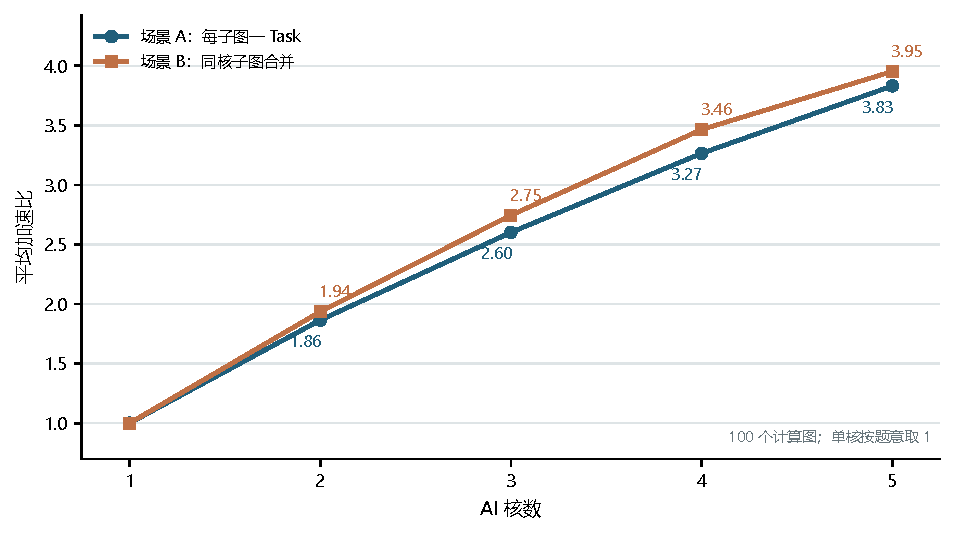
\includegraphics[width=0.83\linewidth]{论文第六章/figures/图6-1_两场景平均加速比.pdf}
\caption{100 图在场景 A、B 下的 1--5 核平均加速比；单核值按题意为 1。}
\label{fig:chapter6-speedup}
\end{figure}
\begin{figure}[htbp]
\centering
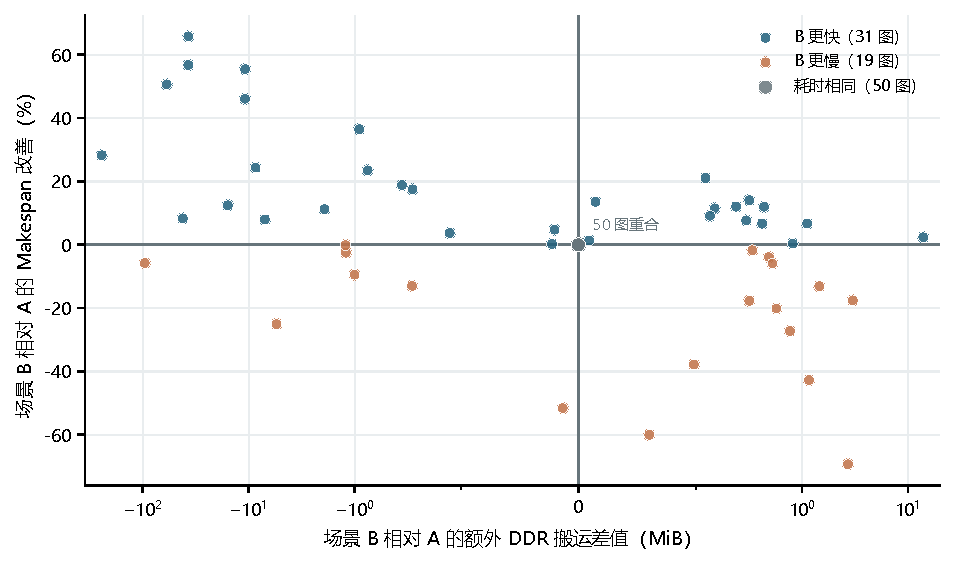
\includegraphics[width=0.83\linewidth]{论文第六章/figures/图6-2_五核耗时与搬运成对比较.pdf}
\caption{五核时场景 B 相对 A 的逐图耗时改善与额外 DDR 搬运变化。横轴用对称对数刻度，零附近保持线性；50 个零差值图在原点重合。}
\label{fig:chapter6-paired}
\end{figure}
图~\ref{fig:chapter6-paired} 同时呈现收益与代价：横轴是额外搬运差、纵轴是 Makespan 的相对改善。模型中的驻留风险只是候选筛选量；论文结果均取自官方程序。
% Q2_RESULTS_END

\subsection{结果的复现边界}
两问的推理程序均以当前图、固定配置和冻结的全局规则为唯一输入，
对每个图/核数从头生成方案；不读取其他图的方案、逐图成绩或评估器输出。
开发阶段可用官方程序检查模型误差，正式方案全部生成并记录
输入、代码和结果哈希后，再由分离脚本作 100 图全量验收。
这一区分保证最终结果是一个可重复运行的算法，而非根据官方反馈
保存的逐例答案。两问的结论只对题目给定数据和硬件配置成立；
换用其他带宽或缓存时应重新分析式~\eqref{eq:chapter6-a-proxy}
及式~\eqref{eq:chapter6-b-rank} 的排序误差。
